\documentclass{beamer}

\usepackage{setspace}
\usepackage{gensymb}
\singlespacing
\usepackage{amsmath}
\usepackage{bm}
\usepackage{cite}
\usepackage{cases}
\usepackage{subfig}
\usepackage{longtable}
\usepackage{multirow}
\usepackage{verbatim}
\usepackage{hyperref}
\usepackage{listings}
\usepackage{color}    
\usepackage{array}    
\usepackage{longtable}
\usepackage{calc}     
\usepackage{multirow} 
\usepackage{hhline}   
\usepackage{ifthen}   
\DeclareMathOperator*{\Res}{Res}

% correct bad hyphenation here
\hyphenation{op-tical net-works semi-conduc-tor}
\def\inputGnumericTable{}                                 %%

\lstset{
%language=C,
frame=single, 
breaklines=true,
columns=fullflexible
}
%\lstset{
%language=tex,
%frame=single, 
%breaklines=true
%}
\hypersetup{
    colorlinks=true,
    linkcolor=black,
    urlcolor=blue,
}
\usetheme{CambridgeUS}

\DeclareMathOperator*{\argmax}{arg\,max}
\DeclareMathOperator*{\argmin}{arg\,min}
\newtheorem{proposition}{Proposition}[section]
\newcommand{\BEQA}{\begin{eqnarray}}
\newcommand{\EEQA}{\end{eqnarray}}
\newcommand{\define}{\stackrel{\triangle}{=}}
\bibliographystyle{IEEEtran}
\providecommand{\mbf}{\mathbf}
\providecommand{\pr}[1]{\ensuremath{\Pr\left(#1\right)}}
\providecommand{\qfunc}[1]{\ensuremath{Q\left(#1\right)}}
\providecommand{\sbrak}[1]{\ensuremath{{}\left[#1\right]}}
\providecommand{\lsbrak}[1]{\ensuremath{{}\left[#1\right.}}
\providecommand{\rsbrak}[1]{\ensuremath{{}\left.#1\right]}}
\providecommand{\brak}[1]{\ensuremath{\left(#1\right)}}
\providecommand{\lbrak}[1]{\ensuremath{\left(#1\right.}}
\providecommand{\rbrak}[1]{\ensuremath{\left.#1\right)}}
\providecommand{\cbrak}[1]{\ensuremath{\left\{#1\right\}}}
\providecommand{\lcbrak}[1]{\ensuremath{\left\{#1\right.}}
\providecommand{\rcbrak}[1]{\ensuremath{\left.#1\right\}}}
\theoremstyle{remark}
\newtheorem{rem}{Remark}
\newcommand{\sgn}{\mathop{\mathrm{sgn}}}
\providecommand{\abs}[1]{\left\vert#1\right\vert}
\providecommand{\res}[1]{\Res\displaylimits_{#1}} 
\providecommand{\norm}[1]{\left\lVert#1\right\rVert}
\providecommand{\mtx}[1]{\mathbf{#1}}
\providecommand{\mean}[1]{\mathbb{E}\left[ #1 \right]}   
\providecommand{\fourier}{\overset{\mathcal{F}}{ \rightleftharpoons}}
\providecommand{\system}[1]{\overset{\mathcal{#1}}{ \longleftrightarrow}}
\newcommand{\cosec}{\,\text{cosec}\,}
\providecommand{\dec}[2]{\ensuremath{\overset{#1}{\underset{#2}{\gtrless}}}}
\newcommand{\myvec}[1]{\ensuremath{\begin{pmatrix}#1\end{pmatrix}}}
\newcommand{\mydet}[1]{\ensuremath{\begin{vmatrix}#1\end{vmatrix}}}
\renewcommand{\vec}[1]{\mathbf{\boldsymbol{#1}}}
% Theme choice:
\newcounter{saveenumi}
\newcommand{\seti}{\setcounter{saveenumi}{\value{enumi}}}
\newcommand{\conti}{\setcounter{enumi}{\value{saveenumi}}}

% Title page details: 
\title[PT-100 ]{An Application of Machine Learning to model a Temperature Sensor(PT100)} 
\author{Lokesh Surana (ES20BTECH11017)}

\begin{document}

% Title page frame
\begin{frame}
    \titlepage
\end{frame}

% Outline frame
\begin{frame}{Outline}
    \tableofcontents
\end{frame}

\section{Introduction}
\begin{frame}{Aim}
    \begin{enumerate}
        \item The modeling of the voltage-temperature characteristics of the PT-100 RTD (Resistance Temperature Detector) using least squares method.
        \item In next slide we have training and validation data. This data have been recorded using voltage readings from serial monitor of arduino and temperature readings from a thermometer. 
    \end{enumerate}
\end{frame}

\section{Data}
\begin{frame}{Training data}
    \begin{table}[ht!]
        \input{tables/training_data.tex}
        \caption{Training data}
        \label{tab:Training data}
    \end{table}
\end{frame}

\begin{frame}{Validation data}
    \begin{table}[!ht]
        \centering
        \input{tables/validation_data.tex}
        \caption{Validation data}
        \label{tab:Validation data}
    \end{table}
\end{frame}

\begin{frame}{Experiment}
    \begin{figure}[!ht]
         \centering
         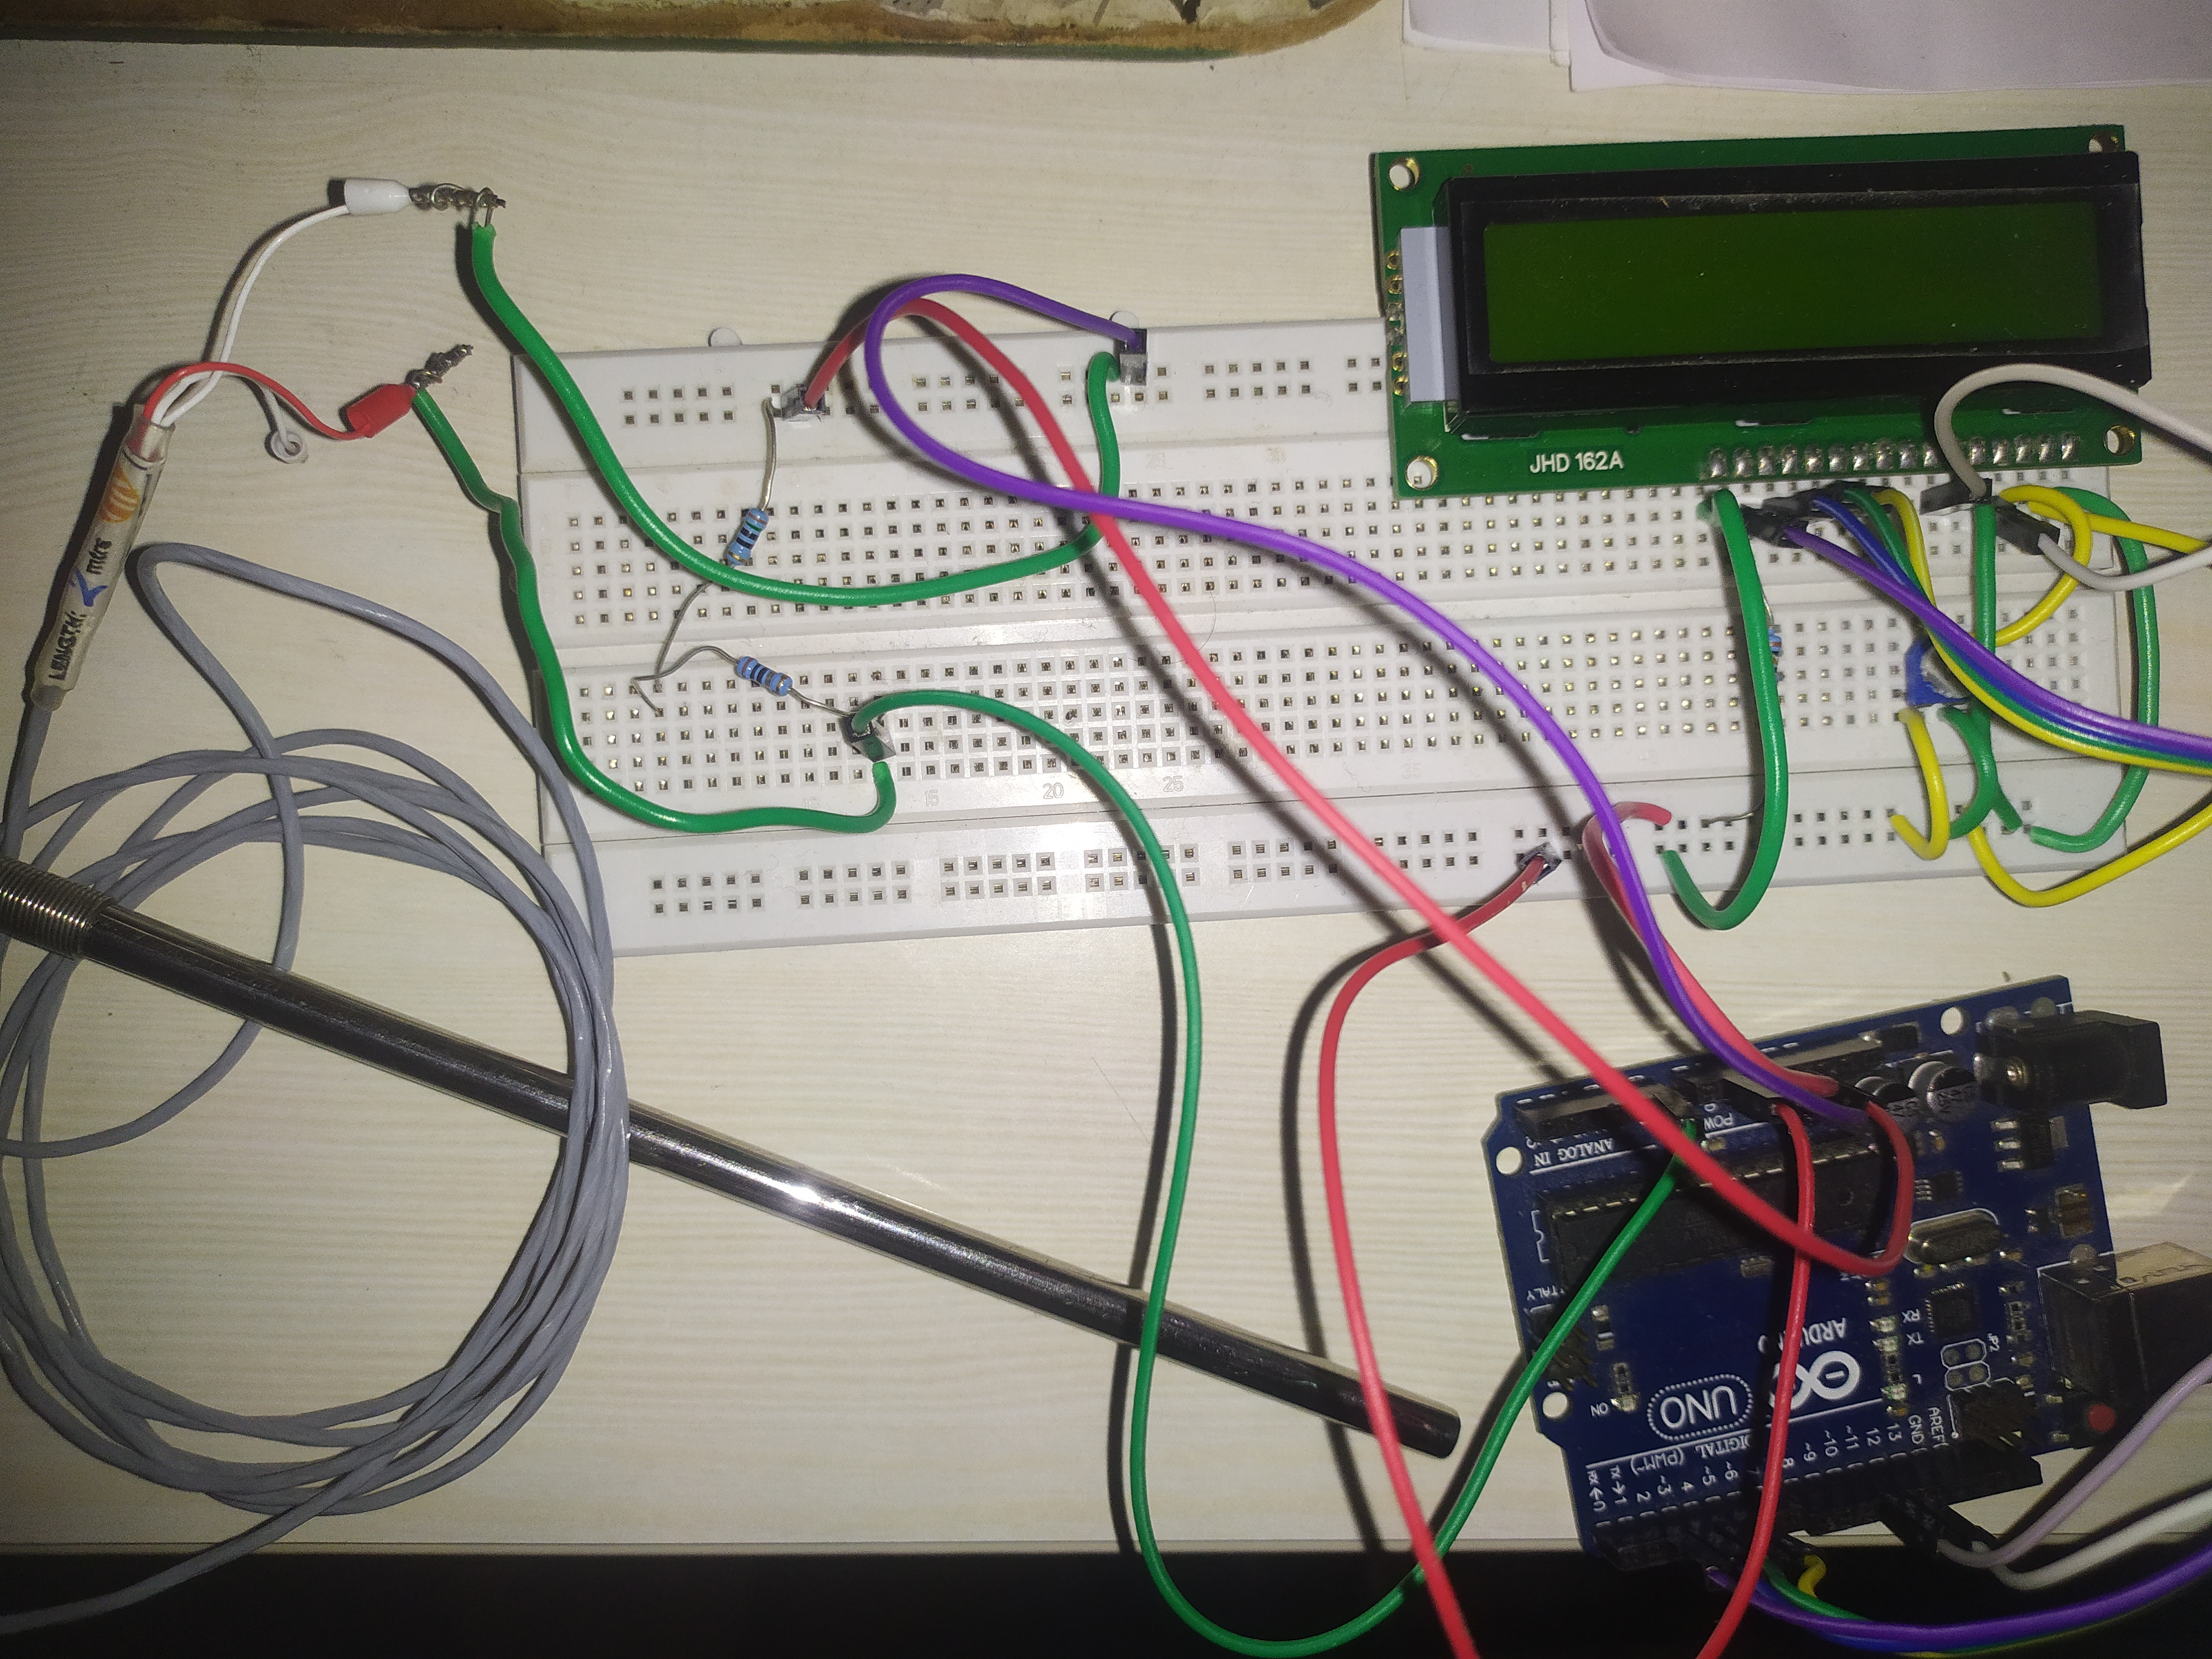
\includegraphics[width=0.6\columnwidth]{figs/setup.jpg}
     \end{figure}
     PT-100 circuit is connected to arduino 3.3V and ground pins. The 200$\Omega$ resistor is being used in circuit. The voltage/sensorvalue is read from A0 pin of arduino.
 \end{frame}

\section{Model}
\begin{frame}{Model}
    For the PT-100, we use the Callendar-Van Dusen equation
    \begin{align}
        V(T)       = V(0)\brak{1+AT+BT^2} \\
        \text{this can be written in the form of } c  = \vec{n}^\top\vec{x}  \\
        c = V(T),\ \vec{n} = V(0)\myvec{1   \\A\\B},\ \vec{x} = \myvec{1\\T\\T^2}
    \end{align}
\end{frame}

\begin{frame}{Model}
    For multiple points,eqn (3) becomes
    \begin{align}
        \vec{X}^\top\vec{n} = \vec{C}                   \\
        \vec{X} & = \myvec{1           & 1 & \ldots & 1 \\T_1&T_2&\ldots&T_n\\T_1^2&T_2^2&\ldots&T_n^2} \\
        \vec{C} & = \myvec{V\brak{T_1}                  \\V\brak{T_2}\\\vdots\\V\brak{T_n}}
    \end{align}
    and $\vec{n}$ is the unknown.
\end{frame}

\begin{frame}{Model}
    We approximate $\vec{n}$ by using the least sqaures method. The Python code
    \texttt{codes/pt100.py} solves for $\vec{n}$.
    The calculated value of $\vec{n}$ is
    \begin{align}
        \vec{n} = \myvec{1.423 \\1.472\times10^{-3}\\9.8158\times10^{-6}}
    \end{align}
\end{frame}

\begin{frame}{Model}
Thus, the approximate model is given by
\begin{align}
    V(T) & = 1.423 + \brak{1.472\times10^{-3}}T \nonumber \\
         & + \brak{9.8158\times10^{-6}}T^2
\end{align}

Equation 8 is in the form of,
\begin{align}
    ax^2 + bx + c=0 
\end{align}

Now, we can use the quadratic formula to find the value of the temperature.
This has been implemented in arduino.

\end{frame}

\end{document}